%!TEX root = ../proyecto.tex
\chapter{Implementación.}
%\section{Breve introducción a CUDA.}
Como comentábamos al principio, CUDA \textit{(Computer Unified Device Arquitecture)} \cite{cuda} es una tecnología propietaria desarrollada por \textit{NVIDIA} y lanzada en junio de 2007, que nos proporciona de un lenguaje de programación general destinado a ser ejecutado en las tarjetas gráficas de la compañia. Para los propósitos de este trabajo y, habitualmente, a la hora de trabajar con CUDA denominaremos como \textbf{\textit{host}} a la CPU que se comunica con la tarjeta gráfica y como \textbf{dispositivo} a la GPU o tarjeta gráfica utilizada. \\

La intercomunicación entre \textit{host} y dispositivo sigue un modelo maestro-esclavo. El \textit{host} actúa como maestro y es el encargado de indicar al dispoistivo el código que ha de ejecutar y de mandarlo a la cola del dispositivo. Además, el \textit{host} tiene la posibilidad de trabajar de forma asíncrona con la GPU mientras la cola de trabajos del dispositivo no esté llena. \\

Es de vital importancia a la hora de trabajar con la GPU de tener en cuenta que:\\
\begin{itemize}
    \item a) La GPU tiene muchos más núcleos \textit{(cores)} que una CPU, lo que nos permite realizar mucha más operaciones en el mismo instante. Sin embargo, esto viene a expensas de un menor número de operaciones por segundo de cada núcleo, ya que para distrutar de la cantidad masiva de núcleos que tiene una GPU es necesario que ésta opere a una frecuencia más baja.

    \item b) La GPU tiene su propia estructura de memoria, que ha de usar para poder realizar operaciones. Dentro de la jerarquía de memoria encontramos memoria RAM similar a la que utiliza la CPU a través de la placa base, así como varios niveles de caché. Además, hemos de tener en cuenta que a la hora de ejecutar algo en la GPU vamos a tener un gasto extra de tiempo por el traspaso de información de CPU a GPU y viceversa. Minimizar la información que ha de traspasarse en ambos sentidos así como intentar que toda la información necesaria sea transferida a la vez para sacar máximo potencial del PCI Express y exprimir al máximo posible el uso eficiente de la memoria caché, que en CUDA es habitualmente realizado mediante el manejo de la ``memoria compartida'' es fundamental para obtener mejores resultados, especialmente, aquellos en los que el cuello de botella es la transferencia de datos.

    \item c) Como la GPU tiene su propia memoria dedicada de un tamaño limitado hemos de hacer hincapié en no utilizar soluciones que generan demasiada complejidad espacial, ya que limitan la escalabilidad de los algoritmos.
\end{itemize}

\subsection{Estructura de hebras, bloques y mallas.}
El \textbf{\textit{kernel}} es un fragmento de código especial destino a ser ejecutado en el dispotivo en el que se indica lo que ha de hacer una hebra.\\

Las \textbf{hebras} son la unidad mínima en la arquitectura CUDA. Cada hebra es ejecutada por un núcleo CUDA. Cada hebra es consciente en tiempo de ejecución de su identificador dentro del bloque así como del identificador del bloque en el que se encuentra y el tamaño del mismo, permitiéndonos así repartir el trabajo en función de dichos valores. El \textbf{bloque} se corresponde a un conjunto de hebras que ejecuta el mismo \textit{kernel} y que pueden cooperar entre sí y, al conjunto de esos bloques, se le denomina \textbf{``grid'' o malla}. Tanto las hebras dentro de un bloque como los bloques dentro de una malla puede tener estructuras unidimensionales, bidimensionales y tridimensionales. Las dimensiones de estas estructuras será indicada por el \textit{host} a la hora de ejecutar el \textit{kernel}.\\

CUDA exige que un mínimo de 32 hebras, denominado \textit{warp}, ejecuten instrucciones a la vez, aunque se hagan cálculos innecesarios así como que todas las hebras de un bloque sean ejecutadas por el mismo \textit{Streaming MultiProcessor}, de ahora en adelante, SM, que es uno de los procesadores en el dispositivo y dispone de un número específico de núcleos CUDA, sus propios registros y su propia caché entre otros.\\

Al lanzar un \textit{kernel} hemos de utilizar al menos un bloque de $N$ hebras. Además, en los casos unidimensionales el número de hebras por bloque está limitado a un máximo que depende de la tarjeta gráfica en cuestión.

\subsection{La memoria compartida.}
Dentro de la tarjeta gráfica, nos encontramos con distintos niveles de memoria. Una vez los datos necesarios han sido traspasados del \textit{host} al dispositivo a través del bus PCI Express, esos datos son almacenados en una memoria DRAM de propósito general del dispositivo. Cuando un \textit{kernel} solicita datos de esta memoria, de manera similar a como ocurre en una CPU, los datos solicitados y los colidantes en memoria son colocados a través de varios niveles de caché, que tiene tamaño más limitado que la memoria DRAM pero con un acceso de lectura y escritura mucho más rápido.\\

La \textbf{memoria compartida} es una abstracción para una región especial de la caché asociada a un bloque que es explícitamente usada por el programador en el \textit{kernel}, agilizando así considerablemente las transferencias de memoria en el dispositivo. En el cuadro \ref{tab:cudamemory}, podemos ver un resumen de los tipos de memoria existentes, dónde se pueden usar y dónde se encuentran dichos datos en el dispositivo.

\begin{table}[ht]
\begin{tabular}{|c|c|c|c|}
\hline
\textbf{Memoria}    & \textbf{Localización}                                           & \textbf{\begin{tabular}[c]{@{}c@{}}Acceso\\ (E = Escribir)\\ (L = Leer)\end{tabular}} & \textbf{\begin{tabular}[c]{@{}c@{}}Existente\\ hasta fin\\ de\end{tabular}} \\ \hline
\textbf{Registro}   & Caché                                                           & Kernel (E/L)                                                                          & Hebra                                                                       \\ \hline
\textbf{Local}      & \begin{tabular}[c]{@{}c@{}}DRAM\\ (Caché tras uso)\end{tabular} & Kernel (E/L)                                                                          & Hebra                                                                       \\ \hline
\textbf{Compartida} & Caché                                                           & Kernel (E/L)                                                                          & Bloque                                                                      \\ \hline
\textbf{Global}     & \begin{tabular}[c]{@{}c@{}}DRAM\\ (Caché tras uso)\end{tabular} & \begin{tabular}[c]{@{}c@{}}Host (E/L)\\ Kernel (E/L)\end{tabular}                     & \begin{tabular}[c]{@{}c@{}}Aplicación\\ o uso de free\end{tabular}          \\ \hline
\textbf{Constante}  & \begin{tabular}[c]{@{}c@{}}DRAM\\ (Caché tras uso)\end{tabular} & \begin{tabular}[c]{@{}c@{}}Host (E/L)\\ Kernel (L)\end{tabular}                       & \begin{tabular}[c]{@{}c@{}}Aplicación \\ o uso de free\end{tabular}         \\ \hline
\end{tabular}
\caption{Resumen de los tipos de memoria en CUDA.}
\label{tab:cudamemory}
\end{table}

\subsection{Python: Numba y CuPy.}
Para desarrollar el código asociado a este proyecto, hemos optado por utilizar \textbf{Python} en vez de los tradicionales C o C++. El uso de \textit{Python} nos permite un desarrollo de los algoritmos más rápido así como el acceso a abstracciones de más alto nivel mediante el uso de la librerías \textbf{\textit{Numba}} y \textbf{\textit{CuPy}},  así como una mayor facilidad para la distribución del código, si se desea, mediante el uso de \textit{PyPI(Python Package Index)}, el repositorio de paquetes para Python. \\

\textbf{Numba} \cite{numba} es un paquete para Python cuyo objetivo es la aceleración compilado fragmentos de código utilizando el compilador LLVM y dando la oportunidad de paralelizar código tanto para la CPU como para la GPU. En concreto, para las GPUs CUDA, proporciona al usuario un subconjunto de las características de CUDA con un nivel de abstracción mayor. Con eso no sólo conseguimos poder trabajar con CUDA desde Python sino, también evitar, si lo deseamos, manejar los traspasos de memoria entre host y dispositivo o la necesidad de indicar todos los tipos a la hora de inicializar un \textit{kernel} entre otras ventajas.
\begin{code}
\begin{minted}[fontsize=\footnotesize]{python}
from numba import cuda
import numpy as np
# Definimos el kernel
@cuda.jit
def aumentar_en_1(un_array):
  # Cogemos el índice de la hebra
    pos = cuda.grid(1)

    # Si el índice está en el rango del array
    # incrementamos su valor
    if pos < un_array.size:
        un_array[pos] += 1

if __name__ == '__main__':
  # Declaramos un array de 10000 ceros
  ejemplo = np.zeros(10000)
  # Calculamos el número de bloques necesario
  bloques = ejemplo.size // 128 + 1
  # Lanzamos el kernel con bloques de 128 hebras
  aumentar_en_1[bloques, 128](ejemplo)
\end{minted}
\captionof{listing}{Kernel para incrementar en 1 los elementos de un array.\\\\}
\label{code:numbaexample}
\end{code}

\textbf{CuPy} \cite{cupy} es otro paquete de Python que, por un lado y de manera similar a Numba, nos permite generar kernels para CUDA en este caso de manera similar a los de C/C++ así como facilidades para generar kernels en los que se implementa reducciones u operaciones elemento a elemento en un array. Por otro lado, proporciona una API similar a la de NumPy pero las operaciones están implementadas utilizando CUDA. Además, CuPy está implementado de manera que permite utilizar directamente sus estructuras de datos sobre kernels de Numba, lo que nos permite combinar elementos de ambos paquetes según nos interese.

\subsection{Spark.}
\textit{Apache Spark} es un \textit{framework} de código abierto y propósito general para sistemas distribuidos de computación en clúster que proporciona una API utilizable desde los lenguajes de programación en Scala, Java, Python y R. El \textit{framework} fundamenta su arquitectura en el \textit{RDD (Resilient Distributed DataSet)}, que es una estructura de datos de sólo lectura distribuida en un clúster de máquinas, mantenida durante toda la computación y con tolerancia a fallos. Además, proporciona otras herramientas de alto nivel como ML/MLib, una librería con algoritmos de \textit{machine learning}.\\

Utilizando la API de Python, podemos combinar el uso de \textit{Spark} y \textit{Numba CUDA} para afrontar problemas de grandes dimensiones, ya que el \textit{RDD} nos permite trabajar con subconjuntos de esos datos posibilitando incluso llevar las implementaciones realizadas a un clúster con múltiples sistemas con dispositivos GPU \textit{CUDA} cont todas las dependencias necesarias instaladas. \\

La distribución de trabajo en Spark se realizará utilizando la transformación \textit{mapPartitions} del \textit{RDD} de \textit{Spark}, que generá un nuevo RDD a partir de los resultados obtenidos al aplicar la función pasada a \textit{mapPartitions} como parámetro a cada una de las funciones.


\section{Proceso de implementación.}
Para realizar la implementación de cada algoritmo hemos realizado un proceso cíclico divido en 3 fases:

\begin{itemize}
	\item \textbf{Análisis} - En la primera iteración, analizar los trabajos relacionados. En las posteriores, analizar los resultados obtenidos del profiler, determinar los cuellos de botella y buscar posibles alternativas para solucionar el problema.
	\item \textbf{Implementación} - Realizar la implementación en CUDA de los cambios o elementos nuevos obtenidos del proceso de análisis.
	\item \textbf{Profiling} - Utilizar el profiler de NVIDIA, \textit{Nsight}, sobre un ejemplo razonable para evaluar el rendimiento del algoritmo.
\end{itemize}

\section{Desarrollo del mapa auto-organizado de Kohonen.}
Para implementar los mapas auto-organizados de Kohonen, primero consideramos la versión tradicional \textit{online} y, posteriormente, tras ver las limitaciones de la primera, evaluamos la versión computada en \textit{batchs}, que ha sido implementada tanto para CPU, usando \textit{NumPy}, como para CUDA, usando \textit{Numba}.

\subsection{Limitaciones del mapa auto-organizado online.}
Mientras que la implementación del mapa auto-organizado \textit{online} fue el punto de partida para la realización de este trabajo, tuvimos que descartar esta versión del algoritmo, ya que, el objetivo de este trabajo es resolver problemas con un gran número de muestras utilizando \textit{CUDA} y \textit{Spark}.\\

En esta versión, en cada iteración, se selecciona una única muestra del conjunto de datos y ésta es evaluada para actualizar los pesos de las neuronas, que serán el punto de partida de la siguiente iteración, limitando a una el número de muestras que pueden procesarse a la vez y, por tanto, secuencializando el proceso.\\

La opción más apropiada para paralelizar esta versión del algoritmo sería procesar una única muestra usando tantas hebras como neuronas tenga el mapa de salida. En ese caso, en cada iteración, cada hebra podría calcular su distancia euclídea de la muestra con los pesos de la neurona asociada a la hebra, usaríamos el algoritmo de la reducción, que explicaremos posteriormente, para encontrar la BMU y, cada hebra, realizaría la actualización de los pesos de su neurona, si ese fuera el caso. Sin embargo, este procedimiento sólo conseguiría ganancias significativas con respecto a su versión para CPU con un mapa de neuronas considerablemente grande, factor que no parece razonable en un algoritmo cuyo principal uso es aprovechar las ventajas que proporciona el \textit{clustering} para procesar cantidades muy grandes de datos.\\

Determinadas estas limitaciones y, dado que nuestro objetivo es evaluar un conjunto con un número de muestras elevado, optamos por implementar la versión del mapa auto-organizado que nos permite evaluar múltiples muestras simultáneamente, conocido como el mapa auto-organizado \textit{batch}.\\


Para el desarrollo de esta versión del algoritmo hemos combinado el uso de \textit{CUDA} mediante \textit{Numba} y \textit{Spark}. En primer lugar, vamos a ver un esquema general del uso de \textit{Spark} para afrontar nuestro algoritmo iterativo y, a continuación, explicaremos en detalle la implementación de los \textit{kernels} para \textit{CUDA}.

\subsection{Uso de Spark.}
\begin{figure}[ht]
\centering
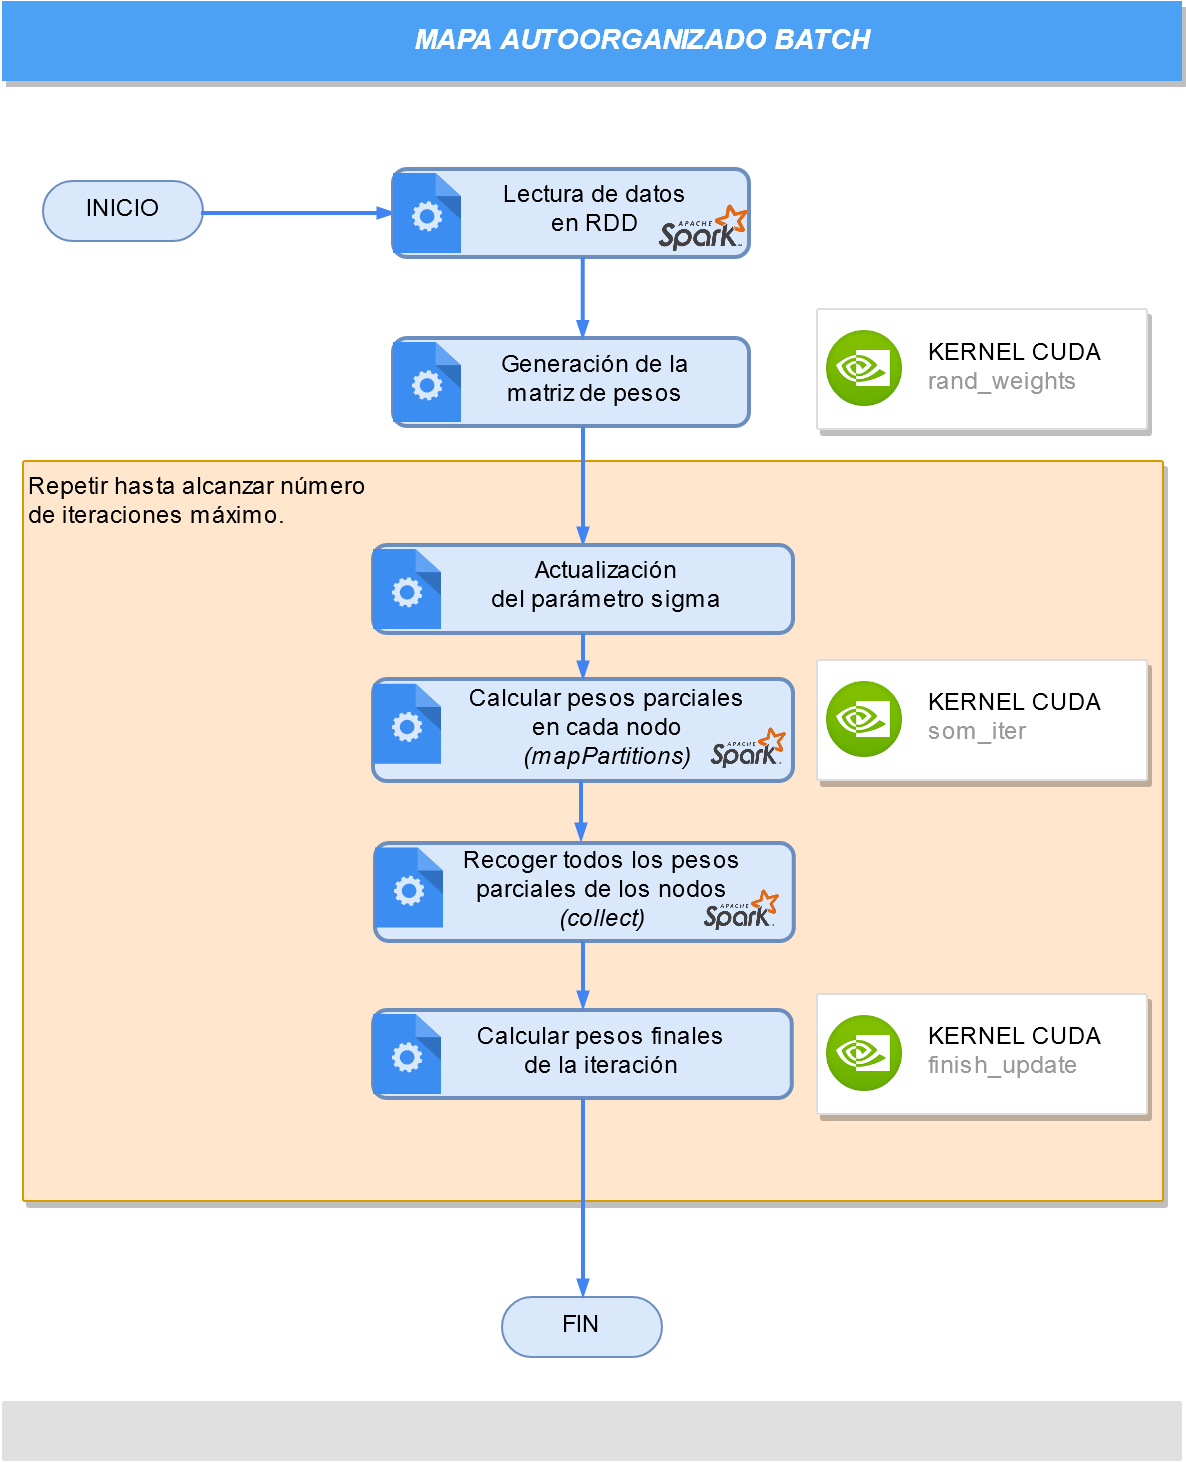
\includegraphics[scale=0.25]{imagenes/flujosparksom.png}
\caption{Diagrama de flujo del mapa auto-organizado desarrollado.}
\label{image:flujosparksom}
\end{figure}

Utilizar \textit{Spark} para implementar este algoritmo nos permite afrontar problemas de tamaños superiores a la capacidad de memoria de nuestro dispositivo, siempre que la memoria necesaria para evaluar una partición del \textit{RDD} quepa en la memoria del dispositivo, y llevar la implementación realizada a un clúster con múltiples nodos, si cada nodo tiene acceso a un dispositivo \textit{CUDA} con todas las dependencias de \textit{software} instaladas.\\


El algoritmo comienza con un  único nodo de \textit{Spark}, utilizando el primer kernel desarrollado, \textit{rand\_weights}, para de esta forma inicializar de manera pseudoaleatoria los valores de la estructura de pesos, en función de una semilla proporcionada por el usuario. Con esta estructura ya generada, empieza el proceso iterativo en el que:
\begin{enumerate}
    \item Calculamos el parámetro de control $\sigma$ para la iteración en función de las ecuaciones correspondientes.

$$\sigma(t) = \left\{
\begin{array}{ll}
\sigma_0e^{-\frac{t}{\tau}} & si \;\;t < z\\
\sigma_f & si  \;\; t\geq z
\end{array}
\right.
$$\\
    \item Utilizando la transformación \textit{mapPartitions}, en cada partición del \textit{RDD} se aplica la función \textit{gpu\_work\_iter}, que encapsula el segundo  \textit{kernel} desarrollado, \textit{som\_iter}. Este \textit{kernel} se encarga de evaluar los pesos parciales para cada neurona en función de las muestras asociadas a la partición del \textit{RDD}. Puesto que la actualización de pesos es una división entre una sumatoria de vectores, con cada vector del tamaño de una muestra, y una sumatoria de números reales, el objetivo de cada partición será calcular esos numeradores y denominadores, a los que nos referiremos de ahora en adelante como numeradores y denominadores parciales.
    $$
 W_{i, j} = \frac{\sum_{k=0}^{f} \delta_f(c, [i,j]) \cdot  X(T_k) }{\sum_{k=0}^{f} \delta_f(c, [i,j])}
$$
    \item Para finalizar la iteración, \textit{Spark} reúne mediante \textit{collect} las numeradores y denominadores parciales obtenidos y, usando el último \textit{kernel} implementado, \textit{finish\_update} obtiene los pesos finales de la iteración.\\
\end{enumerate}

Este proceso, que consta de 3 fases, es realizado hasta alcanzar el número máximo de iteraciones. Hemos de destacar que todas las particiones han de partir de la mismos pesos en cada iteración para realizar los cálculos. Por ello, al inicio de la iteración, es necesario distribuir la matriz de pesos a cada nodo de \textit{Spark} que realiza esos cálculos y, al final de la iteración, reunir todos los numeradores y denominadores parciales en un único nodo, permitiéndonos obtener los pesos finales de la iteración. \\

Para que \textit{Spark} pueda realizar esa distribución a lo largo de un clúster es necesario que, al final de la iteración, se haga la transferencia desde la memoria de dispositivo al \textit{host} ,de los pesos parciales y, al inicio de la iteración, se haga la transferencia desde el \textit{host} al dispositivo de la pesos de las neuronas correspondientes a esa iteración.\\

\begin{code}
\begin{minted}[fontsize=\footnotesize]{python}

def spark_gpu_batch_som(rdd_data, d, max_iters, rows, cols, smooth_iters=None,
                        sigma_0=10, sigma_f=0.1, tau=400, seed=None, tpb=128):
    """
    :param rdd_data RDD con el conjunto de muestras a evaluar.
    :param d Tamaño de una muestra, dimensión del problema.
    :param max_iters Número de iteraciones a realizar.
    :param rows Número de filas en el mapa de neuronas.
    :param cols Número de columnas en el mapa de neuronas.
    :param smooth_iters Número de iteraciones en las que el parámetro
           sigma decrece siguiendo una función gaussiana. 
    :param sigma_0 Valor de sigma inicial.
    :param sigma_f Valor de sigma tras alcanzar la iteración smooth_iters.
    :param tau Valor de tau para la función gaussiana.
    :param seed Semilla pseudoaleatoria para la generación inicial de pesos.
    :param tpb Número de hebras por bloque para la inicialización de pesos y
           la actualización final de los pesos.
    """
    # 1. Declaramos la estructura de los pesos.
    d_weights = cuda.device_array((rows, cols ,d), np.float32)

    # 1.2 Usamos Numba para generar los pesos de forma pseudoaleatoria.
    rng_states = create_xoroshiro128p_states(rows * cols * d, seed=seed)
    rand_weights[(d_weights.size) // tpb + 1, tpb](rng_states, d_weights)
     
    # 1.3 Traemos los pesos de la memoria de la GPU a la memoria del host.
    weights = d_weights.copy_to_host()

    # 2. Inicio del proceso iterativo
    for t in range(max_iters):
        # 2.a Actualizamos sigma en función de los tau y la iteración.
        if smooth_iters is None or t < max_iters:
            sigma = sigma_0 * math.exp((-t/tau))
        else:
            sigma = sigma_f
            
        sigma_squared = sigma * sigma
        
        # 2.b Cálculos parciales con mapPartitions en cada nodo.
        out = rdd_data.mapPartitions(gpu_work_iter(weights, sigma_squared))
        
        # 2.c En un único nodo calculamos las sumas parciales.
        out = out.collect()
        finish_update[rows*cols//tpb + 1, tpb](weights, np.concatenate(out), 
                                               len(out) // 2)
       
    # 3. Devolvemos los pesos obtenidos
    return weights
\end{minted}
\captionof{listing}{Uso de Spark para entrenar el mapa auto-organizado.}
\label{code:somspark}
\end{code}

\subsection{Representación de la estructura de pesos de las neuronas.}
La estructura que contiene los pesos de las neuronas, que durante la ejecución de los \textit{kernels} se encontrará almacenada en la memoria global del dispositivo, se corresponde a un array tridimensional. El primer eje indica la fila que ocupa la neurona en el mapa, el segundo eje indica la columna que ocupa la neurona en el mapa y el último eje la característica del problema a la que queremos acceder.\\

Mientras que nosotros podemos hacer uso de este sistema de indexación tridimensional gracias a Numba, en realidad, en el dispositivo CUDA se trata de un array unidimensional \textit{row-major}.


\begin{figure}[ht]
\centering
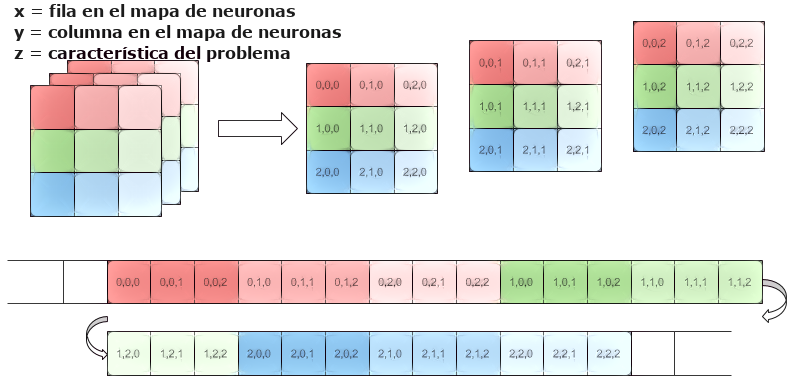
\includegraphics[scale=2.0]{imagenes/row-major.png}
\caption{Representación de un array 3D como un array 1D row-major.}
\label{image:rowmajor}
\end{figure}

\subsection{Kernels implementados.}
\subsubsection{Generación pseudoaleatoria de pesos de neuronas.}
\begin{code}
\begin{minted}[fontsize=\footnotesize]{python}
@cuda.jit
def rand_weights(rng_states, d_weights):
    """
    Kernel para inicializar aleatoriamente la estructura de pesos con 
    valores en el intervalo [0, 1) tomados de una distribución uniforme
    :param rng_states Estados aleatorios.
    :param d_weigths Vector de filas * columnas * d valores que contendrá 
           los pesos asociados a las neuronas.
    """
    # La hebra coge su identificador unidimensional único.
    idx = cuda.grid(1)

    # La hebra calcula en función del su índice 
    # y cocientes y restos de divisiones entereas
    n_rows, n_cols, d = d_weights.shape

    # Cálculo de la fila (eje X).
    row = idx // (n_cols * d)

    # Cálculo de la columna (eje Y).
    col_d = idx % (n_cols * d)
    col = col_d // d
    # Cálculo de la característica (eje Z).
    i = col_d % d
    
    # Sacamos el aleatorio correspondiente.
    if idx < d_weights.size:
        d_weights[row, col, i] = xoroshiro128p_uniform_float32(rng_states, idx)

\end{minted}
\captionof{listing}{Inicialización pseudoaleatoria de los pesos de las neuronas.\\}
\label{code:numbainitweights}
\end{code}

Este proceso (código fuente \ref{code:numbainitweights}) es realizado por el nodo de Spark que controlaría la ejecución del clúster una única vez al inicio del algoritmo, pero utilizando la GPU. \textit{Numba CUDA} nos proporciona herramientas para la generación de valores flotantes en el rango comprendido entre 0 y 1 basadas en el método de Box-Muller. Hemos utilizado esta herramienta para la generación de nuestra matriz de vectores de pesos inicial. Una vez generados, son trasladados de vuelta a la CPU para ser distribuidos a todos los nodos ejecutores de \textit{Spark}. \\

Al lanzar este kernel, se utilizan tantas hebras como números aleatorios (tabla \ref{tab:randkernel}), distribuidos en bloques de un tamaño indicado por el usuario.
\begin{table}[ht]
\begin{tabular}{@{}lll@{}}
\toprule
\textbf{Kernel}        & \textbf{Bloques}                                 & \textbf{Hebras por bloque}                                                                       \\ \midrule
\textbf{rand\_weights} & ($filas$ $\cdot$ $columnas$ $\cdot$ $d$) $//$ $tpb$ + 1 & $tpb$ \\ \bottomrule
\end{tabular}

\textit{\\$d=$ dimensión del problema.\\$tpb=$ hebras por bloque (indicados por el usuario).\\ $//=$ cociente de división entera.}
\caption{Parámetros para el lanzamiento del kernel rand\_weights.}
\label{tab:randkernel}
\end{table}
\newpage
\subsubsection{Cálculo de los numeradores y denominadores parciales.}
\begin{code}
\begin{minted}[fontsize=\footnotesize]{python}
def gpu_work_iter(weights, sigma_squared):
    def _gpu_work(data):
        # 1. Procesamos el dataset
        inp = np.asarray(list(data), dtype=np.float32)
        rows, cols, d = weights.shape
        nneurons = rows * cols
        
        # 2. Pasamos los datos a las memorias del dispositivo
        d_samples = cuda.to_device(inp)
        d_weights = cuda.to_device(weights)
        nums = np.zeros(rows * cols * d, np.float32)
        denums = np.zeros(rows * cols, np.float32)
        d_nums = cuda.to_device(nums)
        d_denums = cuda.to_device(denums)
        
        # 3. Tomamos el número de hebras por bloque
        if nneurons > 1024:
            raise Exception('Número de neuronas superior al límite')
        # Número de hebras necesario para que funcione la reducción.
        tpb = max(64,2**(math.ceil(math.log2(nneurons))))
        # 4. Lanzamos el kernel.
        # Memoria compartida para almacenar una muestra por bloque
        sm_size = 4 * d
        som_iter[N, tpb, 0, sm_size](d_samples, d_weights, d_nums, d_denums,
                                     sigma_squared)
        
        return d_nums.copy_to_host(), d_denums.copy_to_host()
    return _gpu_work
\end{minted}
\captionof{listing}{Función a ejecutar con mapPartitions.\\}
\label{code:somencapsulado}
\end{code}
Una vez obtenidos los pesos iniciales de una iteración, el siguiente paso es utilizar \textit{mapPartitions} para obtener los pesos parciales de cada partición del \textit{RDD}, como veíamos en el código fuente \ref{code:somspark}. La función utilizada en cada partición se denomina \textit{gpu\_som\_iter} y encapsula el lanzamiento del kernel \textit{som\_iter} y las transferencias de memoria entre host y dispositivo en cada iteración.\\

\begin{table}[ht]
\centering
\begin{tabular}{@{}lll@{}}

\toprule
\textbf{Kernel}        & \textbf{Bloques}                                 & \textbf{Hebras por bloque}                                                                       \\ \midrule
\textbf{som\_iter} &   Nº de muestras. & $max(64,2^{techo(\log_2{Nº neuronas})})$ \\ \bottomrule
\end{tabular}
\textit{\\techo=menor número entero mayor o igual que un número real.}
\caption{Parámetros para el lanzamiento del kernel som\_iter.}
\label{tab:iterkernel}
\end{table}

El \textit{kernel som\_iter} es la parte más importante de la implementación del algoritmo y realiza todas las operaciones necesarias para obtener los numeradores y denominadores parciales de la iteración.



\begin{code}
\begin{minted}[fontsize=\footnotesize]{python}
@cuda.jit
def som_iter(d_samples, d_weights, d_nums, d_denums, sigma_squared):
    """
    :param d_samples Conjunto de todas las muestras a evaluar.
    :param d_weigths Vector de filas * columnas * d valores que contendrá 
           los pesos asociados a las neuronas.
    :param d_nums Vector con los numeradores para el cálculo de la fórmula.
    :param d_denums Vector con los denominadores para el cálculo de la fórmula.
    :param sigma_squared Valor de sigma al cuadrado para el cáculo del vecindario.
    """
    nrows, ncols, d = d_weights.shape
    nneurons = nrows * ncols
    
    sample_idx, nueron_idx = cuda.blockIdx.x, cuda.threadIdx.x
    neuron_row, neuron_col = neuron_idx // ncols, neuron_idx % ncols
    blockSize = cuda.blockDim.x
       
    # 0. Declaramos la memoria compartida
    shared_sample = cuda.shared.array(shape=0, dtype=numba.float32)
    shared_distances = cuda.shared.array(shape=1024, dtype=numba.float32)
    shared_idx = cuda.shared.array(shape=1024, dtype=numba.int32)
    
    # 1.a Cada hebra pone una posición de la muestra en memoria compartida.
    # El bucle for permite realizar esto si la dimensión del problema fuese
    # superior al número de neuronas.
    for i in range(d // nneurons + 1):
        i_stride = i * nneurons
        my_pos = i_stride + cuda.threadIdx.x
        # Si la posición que corresponde a la hebra no supera el
        # tamaño de la muestra a cargar.
        if my_pos < d: 
            shared_sample[my_pos] = d_samples[sample_idx, my_pos]
    # Sincronizamos para asegurar que la muestra ha sido cargada.
    cuda.syncthreads()
    
    # 1.b Calculamos las distancias euclídeas que nos corresponden.
    if neuron_idx < nneurons:
        shared_distances[neuron_idx] = 0.0
        for i in range(d):
            i_distance = shared_sample[i] - d_weights[neuron_row, neuron_col, i]
            shared_distances[neuron_idx] += i_distance * i_distance
    # Si hay más hebras que neuronas inicializamos a infinito para la reducción.
    else: 
        shared_distances[neuron_idx] = np.inf
    
    # 1.c Inicializamos el array de índices para la reducción.
    shared_idx[neuron_idx] = neuron_idx
    # Sincronizamos para asegurar los arrays han sido inicializados.
    cuda.syncthreads()    
\end{minted}
\captionof{listing}{Primer fragmento [Cálculo de distancias] de som\_iter.\\}
\label{code:somiter1}
\end{code}

El kernel comienza con la declaración e inicialización de la memoria compartida.\\

En primer lugar, cada hebra contribuye a cargar una característica de la muestra a evaluar por el bloque hasta la muestra ha sido cargada por completo. En segundo lugar, generamos dos arrays adicionales en memoria compartida, que serán utilizados posteriormente para calcular la BMU. Puesto que hemos limitado nuestra implementación a funcionar con un máximo de 1024 neuronas, que es el máximo de hebras por bloque, estos dos arrays serán siempre de esta dimensión. Uno de ellos, que será de \textit{floats} de 32 bits, contendrá las distancias entre la muestra que cargamos en memoria compartida y los pesos de cada neurona del mapa. El segundo, que será de enteros de 32 \textit{bits}, será inicializados con los índices de cada neurona. Para realizar el cálculo de la distancia euclídea, cada hebra calculará su distancia con la neurona que le corresponde y la muestra cargada en memoria compartida. Si hubiese más hebras en el bloque que neuronas en el mapa, el resto de distancias son inicializadas a infinito. \\

Puesto que nuestro siguiente objetivo será encontrar la BMU, es decir, la neurona con menor distancia, no es necesario calcular la raíz cuadrada de la división euclídea, ya que ésta no afecta a la relación de orden. Para encontrar la distancia mínima, utilizamos un algoritmo frecuentemente utilizando en la GPU: \textbf{la reducción}.
\begin{figure}[ht]
\centering
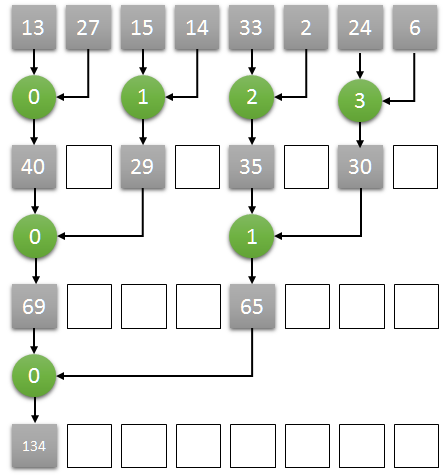
\includegraphics[scale=0.5]{imagenes/parallel_reduce.png}
\caption{Una reducción paralela de una sumatoria.}
\label{image:cudareduction}
\end{figure}
\begin{code}
\begin{minted}[fontsize=\footnotesize]{python}
    # Recorrido de árbol de hojas a la raíz (posición 0)
    if blockSize >= 1024 and neuron_idx < 512:
        if shared_distances[neuron_idx + 512] < shared_distances[neuron_idx]:
            shared_distances[neuron_idx] = shared_distances[neuron_idx + 512]
            shared_idx[neuron_idx] = shared_idx[neuron_idx + 512]
    cuda.syncthreads()
    
    if blockSize >= 512 and neuron_idx < 256:
        if shared_distances[neuron_idx + 256] < shared_distances[neuron_idx]:
            shared_distances[neuron_idx] = shared_distances[neuron_idx + 256]
            shared_idx[neuron_idx] = shared_idx[neuron_idx + 256]
    cuda.syncthreads()
    
    if blockSize >= 256 and neuron_idx < 128:
        if shared_distances[neuron_idx + 128] < shared_distances[neuron_idx]:
            shared_distances[neuron_idx] = shared_distances[neuron_idx + 128]
            shared_idx[neuron_idx] = shared_idx[neuron_idx + 128]
    cuda.syncthreads()
    
    if blockSize >= 128 and neuron_idx < 64:
        if shared_distances[neuron_idx + 64] < shared_distances[neuron_idx]:
            shared_distances[neuron_idx] = shared_distances[neuron_idx + 64]
            shared_idx[neuron_idx] = shared_idx[neuron_idx + 64]
    cuda.syncthreads()
    
    if neuron_idx < 32: # Unroll de warp. No necesitamos sincronizar.
        if shared_distances[neuron_idx + 32] < shared_distances[neuron_idx]:
            shared_distances[neuron_idx] = shared_distances[neuron_idx + 32]
            shared_idx[neuron_idx] = shared_idx[neuron_idx + 32]
        if shared_distances[neuron_idx + 16] < shared_distances[neuron_idx]:
            shared_distances[neuron_idx] = shared_distances[neuron_idx + 16]
            shared_idx[neuron_idx] = shared_idx[neuron_idx + 16]
        if shared_distances[neuron_idx + 8] < shared_distances[neuron_idx]:
            shared_distances[neuron_idx] = shared_distances[neuron_idx + 8]
            shared_idx[neuron_idx] = shared_idx[neuron_idx + 8]
        if shared_distances[neuron_idx + 4] < shared_distances[neuron_idx]:
            shared_distances[neuron_idx] = shared_distances[neuron_idx + 4]
            shared_idx[neuron_idx] = shared_idx[neuron_idx + 4]
        if shared_distances[neuron_idx + 2] < shared_distances[neuron_idx]:
            shared_distances[neuron_idx] = shared_distances[neuron_idx + 2]
            shared_idx[neuron_idx] = shared_idx[neuron_idx + 2]
        if shared_distances[neuron_idx + 1] < shared_distances[neuron_idx]:
            shared_distances[neuron_idx] = shared_distances[neuron_idx + 1]
            shared_idx[neuron_idx] = shared_idx[neuron_idx + 1]
    cuda.syncthreads()
    
    # La mejor neurona se encuentra en la posición 0 del array.
    bmu = shared_idx[0]
    bmu_row, bmu_col = bmu // ncols, bmu % ncols
    cuda.syncthreads()
\end{minted}
\captionof{listing}{Segundo fragmento [Reducción] del kernel som\_iter.\\}
\label{code:somiter2}
\end{code}
  
La reducción puede utilizarse para obtener el resultado de aplicar un operador binario a lo largo de un array, siempre que el operador en cuestión cumpla la propiedad asociativa. En nuestro caso, dicho operador es el mínimo entre dos elementos. Para realizar esta operación de manera eficiente dentro de un bloque, se simula un recorrido hacia arriba sobre un árbol binario balanceado (figura \ref{image:cudareduction}), en el que vamos aplicando la operación sobre los dos hijos y guardando el resultado en el nodo padre, tomando los distancias cargadas en memoria compartida como las hojas y alcanzado el resultado final en la raíz. Por ello, era necesario que el número de hebras por bloque fuese potencia de 2, si teníamos más hebras que neuronas completábamos las distancias con infinito, que actúa como elemento neutro de la operación mínimo, y, añadíamos un array extra con los índices para propagar la posición con el mejor índice mientras hacemos el recorrido. Podemos consultar con más detalle cómo realizar una implementación de una reducción de alto rendimiento en \textit{CUDA} en la referencia bibliográfica \cite{reduction}.\\


Para finalizar el \textit{kernel}, se realiza el cálculo de los numeradores y denominadores parciales. Para ello, cada hebra del bloque se corresponde con una neurona y mide la distancia euclídea que existe entre la posición de la BMU y la posición de la neurona en el mapa. Si esa distancia es menor o igual que el parámetro de control $\sigma^2$, se realiza la suma del vector del numerador con el producto de esa distancia y la muestra guardada en la memoria compartida del bloque y sólo la distancia con el denominador. \\
\begin{code}
\begin{minted}[fontsize=\footnotesize]{python}
# 3. Realizamos la actualización de los pesos.
    if neuron_idx < nneurons:
        dist = (neuron_row - bmu_row) * (neuron_row - bmu_row) + \
               (neuron_col - bmu_col) * (neuron_col - bmu_col)
        # Si estamos dentro del rango de actualización.
        if dist <= sigma_squared:
            hck = math.exp(-dist/(2 * sigma_squared))
            # Guardamos sumatoria del denominador.
            cuda.atomic.add(d_denums, neuron_row * ncols + neuron_col, hck)
            # Guardamos sumatoria del numerador.
            for i in range(d):
                cuda.atomic.add(d_nums, neuron_row*ncols*d + neuron_col*d+i,
                                hck * shared_sample[i])
\end{minted}
\captionof{listing}{Tercer y último fragmento del kernel som\_iter.\\}
\label{code:somiter3}
\end{code}


Puesto que múltiples hebras pueden tener la misma BMU y, por tanto, estar actualizando las mismas posiciones en memoria a la vez se utilizan \textbf{operaciones atómicas}, que evitan las condiciones de carrera que pueda surgir a cambio de una mayor latencia en la operación. Hemos de indicar que, para las operaciones atómicas, necesitamos trabajar con arrays unidimensionales, por lo que hemos de hacer los cálculos de indexación necesarios para acceder a las posiciones de memoria deseadas.

\subsubsection{Cálculo de los pesos finales de la iteración.}
Una vez todos los resultados han sido recopilados en un nodo de \textit{Spark}, lanzamos el \textit{kernel finish\_update}, que realizará la sumatoria de los numeradores parciales y de los denominadores parciales para cada neurona así como la división entre ambos. Si ninguna muestra activó la neurona en cuestión, es decir, la suma de todos sus denominadores parciales es 0, se mantendrán los pesos de la iteración anterior para esa neurona. En caso contrario,  los pesos de la neurona se corresponden con el vector obtenido de la división. Para lanzar este \textit{kernel} se utilizan tantas hebras como neuronas hay en el mapa, divididas en bloque de \textit{tpb} hebras. Cada hebra realiza los cálculos asociados a una neurona.

\begin{table}[ht]
\begin{tabular}{@{}lll@{}}
\toprule
\textbf{Kernel}        & \textbf{Bloques}                                 & \textbf{Hebras por bloque}                                                                       \\ \midrule
\textbf{finish\_update} & (Nº de neuronas // $tpb$ + 1) & $tpb$ \\ \bottomrule
\end{tabular}
\caption{Parámetros para el lanzamiento del kernel finish\_update.}
\label{tab:updatekernel}
\end{table}

\begin{code}
\begin{minted}[fontsize=\footnotesize]{python}
@cuda.jit
def finish_update(d_weights, partials, numParts):
    """
    :param d_weights Array de pesos de neuronas.
    :param partials Array con sumas parciales.
    :param numParts Número de resultados parciales a procesar.
    """
    idx = cuda.grid(1)
    nrows, ncols, d = d_weights.shape
    if idx < nrows * ncols:
        row, col = idx // ncols, col = idx % ncols
        
        # a) Sumamos todos los parciales en el primer array.
        numsize = nrows * ncols * d
        densize = nrows * ncols
        fullsize = numsize + densize
        for i in range(numParts - 1):
            # Suma de numeradores.
            for k in range(d):
                pos = fullsize * i + row * ncols * d + col * d + k
                partials[row * ncols * d + col * d + k] += partials[pos]
            # Suma de denominadores.
            pos = fullsize * i + numsize + row * ncols + col
            partials[numsize + row * ncols + col] += partials[pos]
    
        # b) Si no es 0 el denominador realizamos la división y cambiamos pesos.
        if partials[numsize + row * ncols + col] != 0:
            for k in range(d):
                d_weights[row, col, k] = partials[row*ncols*d + col*d +k] / \
                                         partials[numsize + row * ncols + col]
\end{minted}
\captionof{listing}{Actualización final de la matriz de pesos.\\}
\label{code:ending}
\end{code}

\section{Desarrollo de un modelo de árbol de decisión.}
La implementación del modelo de árbol de decisión se basa en CUDT \cite{cudt}, que a su vez se fundamenta en SPRINT \cite{sprint} y la operación de \textit{scan}.

\subsection{Lista de atributos.}
Una lista de atributos, es una estructura auxiliar, procedente de SPRINT \cite{sprint}, utilizada para representar las clases y los atributos asociados a una muestra. Una lista de atributos tiene una estructura similar a la siguiente tabla:

\begin{table}[ht]
\centering
\begin{tabular}{@{}lll@{}}
\toprule
Valor & Clase & ID Muestra \\ \midrule
2,5   & 0     & 0          \\
4,7   & 0     & 1          \\
0,1   & 1     & 2          \\
1,0   & 1     & 3          \\ \bottomrule
\end{tabular}
\caption{Una lista de atributos sin ordenar.}
\label{tab:ejlistaatributos}
\end{table}

Las columnas de la tabla \ref{tab:ejlistaatributos} son:
\begin{itemize}
    \item \textbf{Valor}, que se corresponde al valor que toma el atributo al que corresponde la tabla en la muestra representada en la fila.
    \item \textbf{Clase}, que se corresponde a la etiqueta de salida asociada a la muestra de la fila.
    \item \textbf{ID Muestra}, que se corresponde al identificador de la muestra. Al principio, se corresponde al número de fila empezando por 0.
\end{itemize}

Una vez esta estructura es generada para cada atributo del problema en cuestión, es ordenada por orden creciente según la columna ``Valor''. En la implementación realizada, se utiliza un array para cada columna.

\subsection{Esquema general del algoritmo implementado.}
\begin{figure}[ht]
\centering
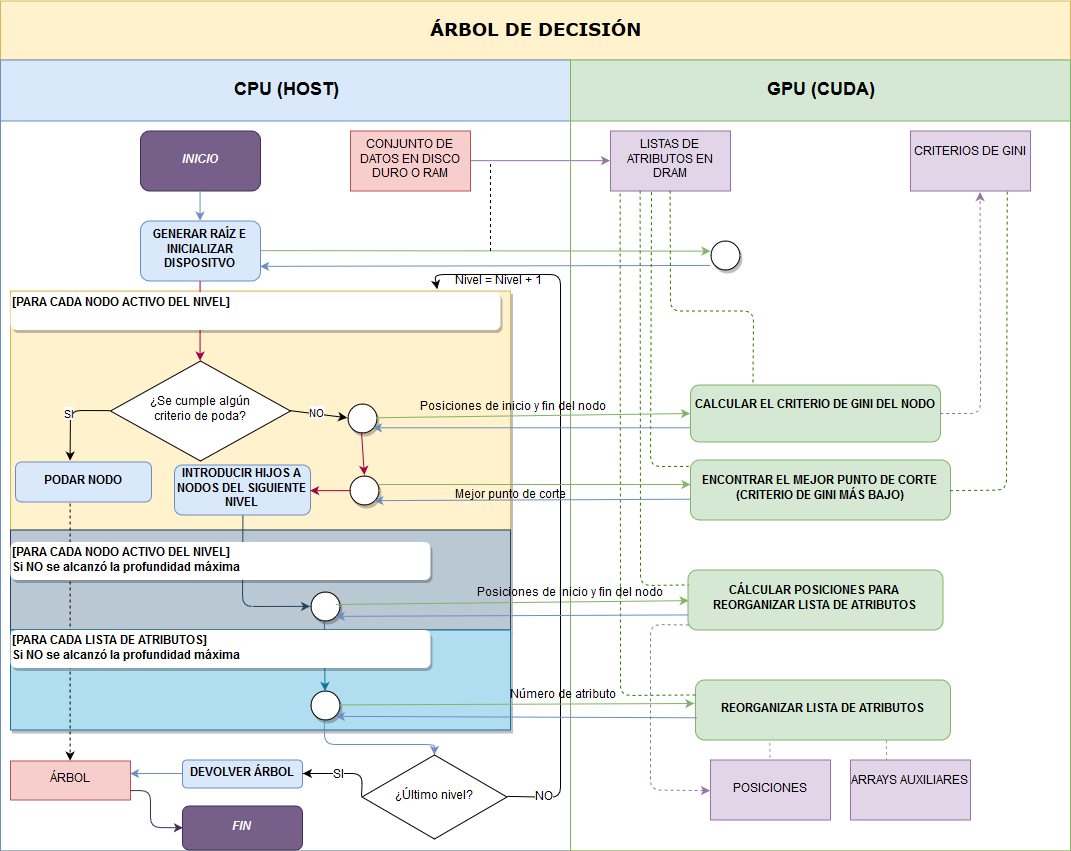
\includegraphics[scale=0.35]{imagenes/esquemadtree.png}
\caption{Diagrama de flujo de la implementación del árbol de decisión.}
\label{img:dtree}
\end{figure}
Al inicio del algoritmo, tras generar las listas de atributos, se genera un nodo raíz que comprende todas las muestras del conjunto. En ese nodo, hemos de encontrar para qué atributo y qué valor realizamos la partición óptima de los datos. Para ello, se consideran todas las listas de atributos y se toma como posible punto de corte el punto medio entre un valor y el siguiente si no se trata del mismo valor. Asociada a cada una de las particiones, se calcula el criterio de Gini. Una vez realizados todos los cálculos, tomamos como punto de corte aquella que menor criterio de Gini nos de. Utilizando ese punto de corte, generamos dos nuevos nodos para la siguiente iteración, uno que contiene todos los puntos menores o iguales que dicho punto de corte y otro con los mayores. Además, dicho punto es el que utilizamos para generar nuestro nodo de decisión en el árbol entrenado.  Este proceso se repite hasta que no quedan nodos por evaluar. Un nodo no ha de ser evaluado si:\\

\begin{enumerate}[a.]
    \item Todos los elementos del nodo pertenecen a la misma clase. En ese caso, en vez de un nodo de decisión, generamos un nodo terminal con la clase correspondiente.
    \item Se ha especificado un criterio de profundidad máxima y dicha profundidad ha sido alcanzada. En ese caso, generamos un nodo terminal con la clase más representativa del nodo.
    \item Se ha especificado un límite para el número de elementos mínimo que puede contener y ha sido alcanzado. En ese caso, generamos un nodo terminal de manera similar al caso anterior.
\end{enumerate}



\subsection{La operación de scan.}
Una de las claves del uso de la lista de atributos, es que, para los problemas de \textbf{clasificación binaria}, que son los únicos que nuestro modelo es capaz de resolver, si codificamos una clase como $0$ (a partir de ahora llamada \textit{clase negativa}) y otra como $1$ (\textit{clase positiva}) si realizamos una suma acumulada sobre el subconjunto de filas de un nodo de la columna ``Clase'' podríamos tener control de cuántos elementos hay en cada clase tanto para todas las particiones. Para realizar la suma acumulada existe una primitiva ampliamente utilizada en el mundo de la GPU denominada \textit{scan}.\\

El \textit{scan} \cite{scan}, suma acumulada o suma prefija, es una operación que utiliza un operador binario, $\oplus$, que cumpla la propiedad asociativa y utilizada sobre un \textit{array} de $n$ elementos. Existen dos formas de realizar el \textit{scan}: inclusivo y exclusivo. El scan inclusivo empieza con el primer elemento del array y va a realizando una suma acumulada. El \textit{scan} exclusivo empieza con el elemento neutro de la operación y realiza una suma acumulada de todos los elementos hasta el penúltimo. En la implementación realizada, hemos utilizado el \textit{scan inclusivo}. Por tanto, para los propósitos de este documento, cada vez que hablemos de \textit{scan}, nos estaremos refiriendo al \textit{scan inclusivo}, que al aplicarla sobre un array, nos devuelve lo siguiente:\\
$$scan([a_0, a_1, a_2, ..., a_{n-1}]) = [ a_0, (a_0 \oplus a_1), (a_0 \oplus a_1 \oplus a_2), ..., (a_0 \oplus a_1 \oplus a_2 \oplus ... \oplus a_{n})]$$

La implementación realizada utilizada operaciones directas sobre \textit{warps}, permitiendo que una ejecución más rápida al realizar todas las operaciones directamente sobre los registros del multiprocesador. De manera más específica el procedimiento realizado es el siguiente.\\

\begin{enumerate}
    \item Se lanza un kernel con una estructura con un número de hebras por bloque predeterminado por el usuario y el mínimo número de bloques para procesar todo el array.\\
    \item El objetivo de cada bloque es calcular su \textit{scan} local.
\end{enumerate}
\begin{enumerate}[{2.}1]
    \item En primer lugar, cada uno de los \textit{warps} del bloque calcula su \textit{scan} local y lo almacena en un array. La operación utilizada para manejar los \textit{warps} es \textbf{shfl\_up\_sync}. Esta operación nos permite realizar una copia y desplazamiento hacia la derecha en el warp en función de una máscara, un valor y un desplazamiento. La máscara nos permite es un conjunto de 32 bits que nos permite indicar cuáles de las 32 hebras han de ser usadas. Para nuestra operación, la máscara está activa para todos las hebras. El valor indica qué valores vamos a utilizar para realizar la operación y ese valor será devuelto en caso de salirnos del rango del warp. Por último, el desplazamiento nos sirve para calcular cuántas posiciones nos hemos de desplazar hacia la derecha. Por ello, empezamos con un desplazamiento de 1 y vamos ampliando siguiendo las potencias binarias inferiores a 32. Para que los resultados ya calculados no sean modificados, nos aseguramos de trabajar sólo con las hebras dentro del warp con índice superior o igual al desplazamiento. Así, al tomar el desplazamiento 1, todos los elementos se suman a su anterior y el primero se mantiene constante. Al tomar el desplazamiento 2, sólo tenemos qué realizar la suma del que había dos posiciones antes, y así, sucesivamente, hasta llegar al último valor. Los últimos valores de cada \textit{scan} local serán guardados en un array en memoria compartida.
    \item Una vez las sumas locales de los warps han sido realizadas, hemos de añadir la suma acumulada obtenida en los \textit{warps} previos para obtener el resultado final del bloque. Para ello, se realiza un \textit{scan} de los \textit{warps} previos, obteniendo el array con las sumas acumuladas previas y estas son aplicadas a los elementos del array correspondientes.\\
\end{enumerate}
\begin{enumerate}[3]
    \item Una vez tenemos el \textit{scan} de cada bloque, hemos de realizar un procedimiento similar para llevar el \textit{scan} local del bloque a todo el array. Esto ha sido realizado, o bien mediante sumas atómicas en el mismo \textit{kernel}, que son más lentas que las operaciones normales, o bien combinando el trabajo con otros \textit{kernels} que tenían que ser lanzados de forma independiente.

\end{enumerate}



\subsection{Cálculo del criterio de Gini.}
Dado que sólo vamos a calcular el criterio de Gini para problemas de clasificación binaria hemos simplificado el mismo para ahorrarnos algunas operaciones a la hora de realizar el cálculo:

$$CRITERIO(A,v) = \frac{|i: A_i \leq v|}{N} \cdot GINI(|i: A_i \leq v|) + \frac{|i: A_i > v|}{N} \cdot GINI(|i: A_i > v|)$$

$$GINI(D) = 1 - \frac{T_D^2}{N_D^2} - \frac{F_D^2}{N_D^2}$$

Siendo $N_D$ el total de las muestras en el nodo $D$, $T_D$ el total de muestras pertenecientes a la clase positiva y $F_D$ el total de muestras pertenencientes a la clase negativa. Tenemos que:

$$F_D = N_D - T_D$$
Sustituyendo obtenemos que:

$$GINI(D) = \frac{N_D^2-T_D^2- (N_D - T_D)^2}{N_D^2} = \frac{N_D^2 - T_D^2 - (N_D^2+T_D^2 - 2 N_D T_D)}{N_D^2}$$
$$GINI(D) = \frac{-2T_D^2 + 2N_DT_D}{N_D^2} = 2 \frac{T_D(N_D-T_d)}{N_D^2}$$

$$CRITERIO = \frac{N_\leq}{N}\frac{2T_\leq(N_\leq - T_\leq)}{N_\leq^2} + \frac{N_>}{N}\frac{2T_>(N_> - T_>)}{N_>^2}$$
$$CRITERIO = \frac{2}{N}\Big(\frac{T_\leq(N_\leq - T_\leq)}{N_{\leq}} + \frac{T_>(N_> - T_>)}{N_>}\Big)$$

Puesto que además, no es de nuestro interés el valor específico sino obtener el valor óptimo, podemos ahorrarnos la multiplicación por $\frac{2}{N}$. Así pues, calculamos el criterio de la siguiente manera:

$$CRITERIO' = \Big(\frac{T_\leq(N_\leq - T_\leq)}{N_{\leq}} + \frac{T_>(N_> - T_>)}{N_>}\Big)$$

El valor de $CRITERIO'$ oscilará entre 0 y $\frac{N}{2}$ y buscaremos siempre obtener el mínimo valor para este criterio. Dicha búsqueda se realizará de manera similar a la realizada para el modelo anterior con una reducción para encontrar el índice mínimo en cada nodo.

\subsection{Reorganización de la listas de atributos.}
Para finalizar la evaluación de los nodos de un nivel podemos volver a aprovechar la operación de \textit{scan} para reorganizar el orden de los elementos de la lista de atributos sin necesidad de ejecutar ningún algoritmo de ordenación.\\

 Una vez se ha seleccionado la combinación de mejor lista de atributos para un nodo y su punto de corte, puesto que esta lista ya estaba ordenada, todos los elementos hasta el punto de corte pertenecen al nodo hijo izquierdo y los posteriores al nodo hijo derecho. Además, puesto que tenemos en la lista de atributos el campo ``ID Muestra'', podemos generar fácilmente un array de booleanos donde cada elemento indica si la muestra con el ID asociado a su posición.\\

 Si aplicamos la operación de \textit{scan} sobre este array auxiliar, la suma acumulada en cada posición nos indica el número de elementos que pertenecen al nodo hijo codificado con la etiqueta positiva. Por lo que, partiendo de que previamente estaban ordenados podemos hacer la subdivisión y mantener el orden teniendo en cuenta que:\\

 \begin{enumerate}
    \item Si el elemento en cuestión pertenece al nodo hijo izquierda (codificado como positivo en el array auxiliar), su nueva posición en la lista de atributos sería la suma acumulada obtenida en el array auxiliar menos uno (para que el primer índice sea el 0).
    \item En caso contrario, la nueva posición es el número total de elementos en el nodo hijo izquierda (para que ambos queden separados) más la diferencia de ese total de elementos del nodo hijo izquierda con la suma acumulada del array auxiliar (que nos indicaría cuántos elementos de la clase negativa llevamos hasta el momento) menos uno (porque la indexación empieza en 0).
 \end{enumerate}

\subsection{Representación del árbol.}
Durante el proceso de entrenamiento, la necesidad de lanzar múltiples \textit{kernels} al no disponer desde Python de paralelismo dinámico ha hecho que hayamos optado por almacenar tanto la estructura del árbol de salida como la que controla los nodos a evaluar en la CPU.\\

La estructura que controla los nodos a evaluar es una lista que contiene todos los nodos activos del nivel y, cada elemento de la lista, es una tupla que contiene el inicio, el fin del nodo y el índice correspondiente a ese nodo si recorremos el nivel de izquierda a derecha y no se hubiese podado ningún elemento. Puesto que es necesario que la CPU acceda a estos datos para controlar el flujo de ejecución de los \textit{kernels} no tiene sentido almacenar la misma en la GPU. \\

En el caso del árbol de salida, deberíamos de almacenar una estructura que nos permita almacenar los valores y atributos de un punto de corte y la clase de salida, si fuese un nodo terminal. Esta estructura podría ser almacenada por la GPU y podría ayudar a obtener mejores resultados, especialmente si disponemos de paralelismo dinámico. Sin embargo, tanto el momento en el que se poda un nodo como en el que se calcula el mejor punto de corte suponen la finalización de un \textit{kernel} y la devolución de datos a la CPU, por lo que añadir un dato más no supondría el cuello de botella si no la mera parada para realizar la transferencia. Además, en temas de escalabilidad, no almacenar la estructura del árbol en la GPU evita un gasto considerable de memoria RAM del dispositivo en un algoritmo con una gran complejidad espacial debido al uso de las listas de atributos en la GPU, que añaden dos campos extras para cada combinación de muestra y atributo que no sea la etiqueta de salida.\\

La representación utilizada para el árbol de salida es una lista de diccionarios de tuplas. En primer lugar, la lista tendrá tantos diccionarios como niveles de profundidad tenga el árbol, siendo el nivel 0 la raíz. El diccionario tendrá como clave de entrada un valor numérico, que se corresponderá a la posición que ocuparía el nodo si recorremos el nivel de izquierda a derecha y no se hubiese podado ningún elemento. De esta manera, si nos encontramos ante un nodo de decisión, sus hijos se encontrarían en el diccionario de la siguiente posición de la lista y sus índices de acceso serían el doble del índice de acceso de su padre o el doble del índice de acceso de su padre más 1, dependiendo de a cuál de los dos hijos queramos acceder. Por último, la descripción que se encuentra en en el diccionario para una clave de acceso es una tupla. Dicha tupla indica si el nodo es decisión o terminal. En el caso de ser un nodo de decisión, dispone de campos para el atributo y su valor de corte. En el caso de ser un nodo terminal, dispone de un campo que indica la clase con la que etiquetar la muestra. 

\subsection{Uso de Spark.}
Este modelo, al requerir la evaluación independiente de múltiples nodos, como podremos comprobar posteriormente, no escala bien con la generación de árboles profundos o completos. Es por eso que, a la hora de integrar \textit{Spark} en la solución, en vez de generar un único árbol, vamos a generar un \textit{random forest}, es decir, vamos a subdividir la muestras de entrenamiento aleatoriamente de tal manera que cada partición de \textit{Spark} entrenará un árbol y, una vez los árboles han sido entrenados, una muestra a clasificar será evaluada por todos los árboles. La clase de la muestra se corresponderá a la clase que ha sido seleccionada en el mayor número de árboles. \\

Esta solución nos permite, por un lado, reducir problemas de sobreajuste, y, por otro, conseguir precisiones competentes sin necesidad de generar árboles completos u otros sistemas de poda más complejos y evitar los problemas de sincronización y comunicación que generaría el entrenamiento de un único árbol como que todos los nodos de \textit{Spark} tendrían que tener una copia de las listas de atributos y, al terminar cada nivel de profundidad debería de plantearse una estrategia para reordenar las listas de atributos y volver a distribuir los cambios a todos los nodos.

